\documentclass[a4paper, 12pt]{article}

\usepackage{ucs}
\usepackage[utf8x]{inputenc}
\usepackage[T1]{fontenc}
\usepackage[french]{babel}

\usepackage{microtype}

\usepackage{lmodern}
\usepackage[bitstream-charter]{mathdesign}

\usepackage[margin=1.5cm]{geometry}

\usepackage{color}
\definecolor{blue}{rgb}{0.38,0.58,0.81}
\definecolor{green}{rgb}{0.47,0.72,0.33}
\definecolor{red}{rgb}{0.91,0.34,0.32}
\definecolor{frame}{rgb}{0.70,0.70,0.70}
\definecolor{grey}{rgb}{0.97,0.97,0.97}

\PrerenderUnicode{ώ}

\usepackage{hyperref}
\hypersetup{
  pdftitle={Devoir de programmation multi-cœurs},
  pdfsubject={},
  pdfauthor={Hervé Blocier - Damien Gombault},
  colorlinks,
  citecolor=black,
  filecolor=black,
  linkcolor=black,
  urlcolor=blue
}

\usepackage[pdftex]{graphicx}

\usepackage{listings}
\lstset{
   tabsize=1,
   frame=single,
   breaklines=true,
   basicstyle=\ttfamily \small,
   rulecolor=\color{frame},
   backgroundcolor=\color{grey},
   framexleftmargin=5mm,
   xleftmargin=5mm,
}

\begin{document}

\thispagestyle{empty}

\begin{center}
\vspace*{\fill}

\hrule
\vspace{1cm}
{\Huge \textbf{Devoir de programmation multi-cœurs}\\}
\vspace{1cm}
\hrule

\vspace{2cm}

\includegraphics[width=5cm]{includes/png/logo-univ.png}
\vspace{2cm}

{\Large
\textbf{Étudiants} \\
Hervé BLOCIER \\
Damien GOMBAULT \\
}

\vspace{4cm}

\large{18 mars 2009\\}

\vspace*{\fill}
\end{center}

\newpage

\renewcommand{\contentsname}{Sommaire}
\setcounter{tocdepth}{2}
\tableofcontents
\newpage

\section{Description de l'archive}

\begin{itemize}
\item \texttt{doc/} : ce document et ses sources au format
  {\fontfamily{lmodern}\LaTeX}
\item \texttt{doxygen/} : la documentation Doxygen du projet
\item \texttt{src/} : les sources C++ du projet
\item \texttt{doxygen.conf} : le fichier de configuration pour la
  génération de la documentation Doxygen
\item \texttt{Makefile} : le \texttt{Makefile} qui permet de compiler
  le projet
\item \texttt{test.sh} : un script shell qui permet de tester le
  programme \texttt{strassen} avec les outils fournis avec le devoir
\end{itemize}

\section{Compilation}

Pour compiler le projet, il suffit simplement de taper la commande
suivante à la racine du projet :

\begin{lstlisting}
$ make
\end{lstlisting}
% $

Par défaut, le support OpenMP est activé. Si vous souhaitez le
désactiver, vous devez modifier la première ligne du fichier
\texttt{Makefile} et remplacer \texttt{OPENMP=1} par
\texttt{OPENMP=0}. Nettoyez ensuite les sources avec la commande
\texttt{make clean} puis lancez de nouveau la compilation avec la
commande \texttt{make}. \\

Après compilation, trois nouveaux exécutables sont créés.

\paragraph{\texttt{generate}}

Ce programme permet de générer de façon aléatoire une matrice et de
l'enregistrer dans un fichier. Il est possible de choisir la taille de
la matrice.

\begin{lstlisting}
Usage: ./generate size outputfile
\end{lstlisting}

\paragraph{\texttt{benchmark}}

Ce programme permet de tester les performances de l'algorithme
implémenté. Il génère des matrices de façon aléatoire et effectue leur
multiplication en utilisant l'algorithme de Strassen. Il est possible
de choisir la taille des matrices générées et le nombre de
multiplications à effectuer.

\begin{lstlisting}
Usage: ./benchmark size iteration
\end{lstlisting}

Il est recommandé d'utiliser la commande \texttt{time} interne au
shell pour mesurer le temps d'exécution du programme :

\begin{lstlisting}
$ time ./benchmark 256 1
./benchmark 256 1  4,87s user 0,03s system 96% cpu 5,104 total
\end{lstlisting}
% $

\paragraph{\texttt{strassen}}

Ce programme effectue la multiplication de Strassen de deux matrices
lues à partir de deux fichiers en entrée et enregistre le résultat
dans un autre fichier.

\begin{lstlisting}
Usage: ./strassen inputfile1 inputfile2 outputfile 
\end{lstlisting}

\pagebreak

\section{Test}

Pour tester le programme, il faut d'abord copier à la racine du projet
les exécutables \texttt{mult} et \texttt{compare} fournis avec le
devoir. Il suffit ensuite d'utiliser le script shell \texttt{test.sh}
et lui spécifier une taille de matrice :

\begin{lstlisting}
$./test.sh 256
Generating 256-sized matrix 1... Ok
Generating 256-sized matrix 2... Ok
Computing strassen algorithm... Ok
Computing normal algorithm... Ok
Comparing results... Ok
\end{lstlisting}
% $

\section{Implémentation}

Nous avons développé plusieurs implémentations de l'algorithme de
Strassen mais nous présentons uniquement notre version la plus
performante qui est développée en C++ avec OpenMP. Nous avons
également essayé de dérécursiver l'algorithme de Strassen mais nous ne
sommes pas arrivé à des résultats satisfaisants. Nous avons également
essayé d'implémenter une version en utilisant les \textit{threads} POSIX. \\

Nous avons choisi le C++ afin d'obtenir une implémentation de haut
niveau proche de l'algorithme original. Nous utilisons par exemple la
surcharge des opérateurs \texttt{*}, \texttt{+} et \texttt{-}. Ceci
nous permet d'avoir un code plus concis et facile à lire. \\

Le principal inconvénient des implémentations haut niveau est qu'ils
ne sont généralement pas très performants. Nous avons donc cherché à
obtenir un compromis intéressant entre haut niveau et performances.
Nous avons donc cherché à optimiser cet algorithme en utilisant
certaines fonctionnalités avancées du C++ comme les \texttt{rvalue
  references}\footnote{\url{http://www.artima.com/cppsource/rvalue.html}}.
Cette technique permet d'éviter un nombre important de recopies et
ainsi augmenter de façon conséquente les performances. Une version
récente du compilateur GCC est ainsi requise. Le projet a uniquement
été testé avec la version 4.3 de ce compilateur. \\

Concernant la parallélisation, nous avons préféré utiliser OpenMP. Il
nous permet de garder un code concis et facile à lire. \\

Nous avons tout d'abord tenté de paralléliser les petites opérations
sur les matrices (les additions et les soustractions) mais cette
version était beaucoup plus lente à cause de l'\textit{overhead}
provoqué par la création des \textit{threads}. Le système passait
beaucoup plus de temps à gérer les \textit{threads} qu'à faire les calculs. \\

Nous avons donc changé de méthode et tenté de paralléliser l'exécution
récursive de l'algorithme de Strassen. Ceci est permis grâce à
l'utilisation du \textit{nested parallelism} d'OpenMP. Nous avons
limité ce parallélisme au niveau de la récursion par la formule $
\frac{\log_2 \mathrm{taillematrice}}{2} $. Cette technique nous permet
d'obtenir un bon compromis entre le nombre de calculs effectués et le
nombre de \textit{threads} créés. Ceci permet ainsi d'augmenter les
performances de l'algorithme. \\

Nous pourrons dans un futur proche utiliser les tâches
(\textit{tasking}) d'OpenMP 3.0 à la place du \textit{nested
  parallelism} d'OpenMP 2.5. Il s'agit d'une autre méthode plus
performante pour exploiter le parallélisme imbriqué. Actuellement,
cette fonctionnalité n'est pas implémentée dans GCC 4.3.

\pagebreak

\section{Performances}

Nous avons effectué quelques tests de performance de notre projet.
Nous avons lancé 5 exécutions du programme avec OpenMP puis sans
OpenMP avec des tailles de matrices différentes et nous avons ensuite
fait la moyenne des temps obtenus. Voici les résultats obtenus (en
secondes) :

\begin{center}
\begin{tabular}{|l|r|r|r|r|r|r|}
\hline
\textbf{Taille } & \textbf{64} & \textbf{128} & \textbf{256} & \textbf{512} & \textbf{1~024} & \textbf{2~048} \\ \hline
\texttt{\textbf{OPENMP=0}} & 0,102 & 0,697 & 4,872 & 34,086 & 238,524 & 1~677,14 \\ \hline
\texttt{\textbf{OPENMP=}1} & 0,104 & 0,641 & 4,384 & 30,586 & 213,578 & 1~496,15 \\ \hline
& \textcolor{red}{-1,74\%} & \textcolor{green}{8,67\%} & \textcolor{green}{11,13\%} & \textcolor{green}{11,44\%} & \textcolor{green}{11,68\%} & \textcolor{green}{12,10\%} \\ \hline
\end{tabular}
\end{center}

\begin{center}
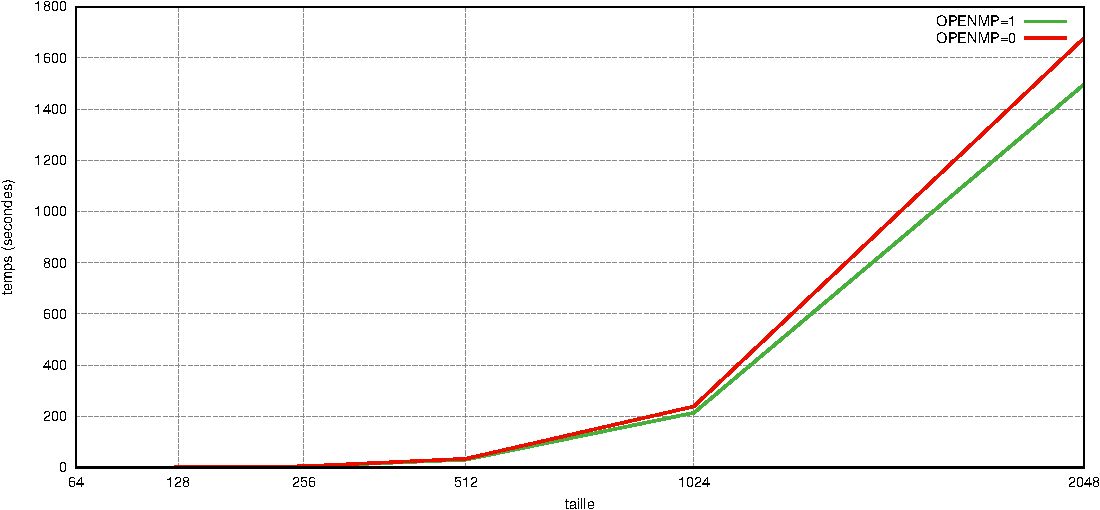
\includegraphics[width=\textwidth]{includes/pdf/benchmark.pdf}
\end{center}

On peut donc remarquer que notre version OpenMP apporte un gain
d'environ 11\% par rapport à la version sans OpenMP. Nous pouvons
également remarquer que le gain semble légèrement augmenter avec la
taille de la matrice. \\

Nous avons effectué nos tests avec un Pentium Dual-Core T2080 (1,73
GHz / 1 Mio de Cache L2). Nous n'avons pas pu tester notre application
avec plus de cœurs car nous n'avions pas de machine mieux équipées à
disposition.

\end{document}